\documentclass[11pt]{article}

\usepackage{amssymb,amsmath,amsfonts,eurosym,geometry,ulem,graphicx,caption,color,setspace,sectsty,comment,footmisc,caption,natbib,pdflscape,subfigure,float,array,hyperref}
\usepackage{booktabs}
\usepackage{tabularx}
\usepackage{hyperref}
\usepackage{enumitem}
\usepackage{indentfirst}
\usepackage{threeparttable}
\usepackage{subfigure} 
\usepackage{longtable}
\normalem
\usepackage[dvipsnames]{xcolor}
\definecolor{myblue}{RGB}{5,90,140}
\hypersetup{
	colorlinks=true,
	urlcolor=myblue
}
\hypersetup{
	colorlinks=true,
	linkcolor=myblue
}
\hypersetup{
	colorlinks = true,
	%	linkcolor = blue,
	anchorcolor = black,
	citecolor = black,
	filecolor = blue,
	%	urlcolor = blue
}

\onehalfspacing
\newtheorem{theorem}{Theorem}
\newtheorem{corollary}[theorem]{Corollary}
\newtheorem{proposition}{Proposition}
\newenvironment{proof}[1][Proof]{\noindent\textbf{#1.} }{\ \rule{0.5em}{0.5em}}
\newtheorem{hyp}{Hypothesis}
\newtheorem{subhyp}{Hypothesis}[hyp]
\renewcommand{\thesubhyp}{\thehyp\alph{subhyp}}

\newcommand{\red}[1]{{\color{red} #1}}
\newcommand{\blue}[1]{{\color{blue} #1}}

\newcolumntype{L}[1]{>{\raggedright\let\newline\\arraybackslash\hspace{0pt}}m{#1}}
\newcolumntype{C}[1]{>{\centering\let\newline\\arraybackslash\hspace{0pt}}m{#1}}
\newcolumntype{R}[1]{>{\raggedleft\let\newline\\arraybackslash\hspace{0pt}}m{#1}}
\newcounter{file}
\newcommand{\file}{\refstepcounter{file}(\arabic{file})}
\geometry{left=1.0in,right=1.0in,top=1.0in,bottom=1.0in}
\setlength{\parindent}{2em} 

\begin{document}

\begin{titlepage}

\title{Conference Call Code Manual}
\date{\today}
\author{Sixun Tang \\ Valerii Baidin}
\maketitle
\begin{abstract}
This manual gives a detailed description of the whole process of exporting and processing conference calls for various textual analysis practices.


%\vspace{0in}\\
%\noindent\textbf{Keywords:} key1, key2, key3\\
%\vspace{0in}\\
%\noindent\textbf{JEL Codes:} key1, key2, key3\\\
\bigskip
\end{abstract}

\setcounter{page}{0}
\thispagestyle{empty}
\end{titlepage}

\pagebreak
\newpage
	
\doublespacing
\tableofcontents

\newpage

\section{Overview}
\par This manual describes the whole process of exporting and processing conference calls for textual analysis from Thomson Streetevents database, which is available from Thomson One (Booth access). Thomson One updates latest conference calls on a regular basis and we need to rerun the codes to capture the latest call scripts. The main challenge is that the platform does not support scraping and poses a strict restriction on the maximum number of conference calls exported every time. As a result, we write automatic codes imitating the downloading action to circumvent the obstacle. Additionally, we use tools from Booth Mercury server and Julia codes to transfer the raw pdf files to usable text files stored in csv files. Finally, we match the conference calls with standard firm identifier, i.e., gvkey from Compustat, to facilitate linking to other firm data sets.

\section{Data Structure}
\par Currently we have already downloaded and processed conference calls from 01/08/2001 to 04/05/2021. The full data are stored in ConferenceCallData on Kilian's serve folder. The data are divided into five folders. The folders are organized by steps of the whole process, which we'll describe in details later.
\begin{enumerate}
	\item \textbf{RawScripts}: Raw pdf files and OCR-transferred txt files of the original pdf files, i.e., each set of conference calls contain two files, one pdf and one txt.
	\item \textbf{List}: xls files which contains the basic information of each conference call, including title, subtitle, report number, date, time, etc..
	\item \textbf{CsvScripts}: Usable csv scripts. The csv file is processed by combining basic information from the .xls file and scripts from .txt file. These csv files could be directly fed to Python/Julia codes.
	\item \textbf{FileRecord}: The records of conference calls in each time period (dta file). Additionally, there are two csv files containing the bad conference calls that could not be processed from txt files.We ran three rounds of collection and there were several bad conference calls in the first two round.
	\item \textbf{FirmNameMatching}: csv files containing basic information of conference call and matched firm names from Compustat. The file could be linked to scripts using report number. For the first round, we have separate csv files for each year (2001-2020) and a total file of matched records with $\geq$ 90 matching probability. For round two and round three, the matching files are named as "*\_202010" and "*\_202104" respectively.
\end{enumerate}

\section{Step 1: Downloading Raw Data}
\par There are several obstacles preventing us from exporting conference calls from the platform:
\begin{enumerate}
	\item Each page will only show 50 conference calls.
	\item A maximum of 2,000 conference calls will be presented for every search.
	\item Web drivers are prohibited
\end{enumerate}
\par To circumvent these obstacles, we design a series of codes to imitate the human downloading action. The summary of the procedure are shown in the following figures.
\begin{enumerate}
	\item Use Internet Explorer (no other browers are allowed) to access Thomson One (\url{proxy.uchicago.edu/login/thomsonone}).
	\item Go to \textit{Screen Analysis}-\textit{Research}
	\begin{figure}[H]
	\begin{center}
	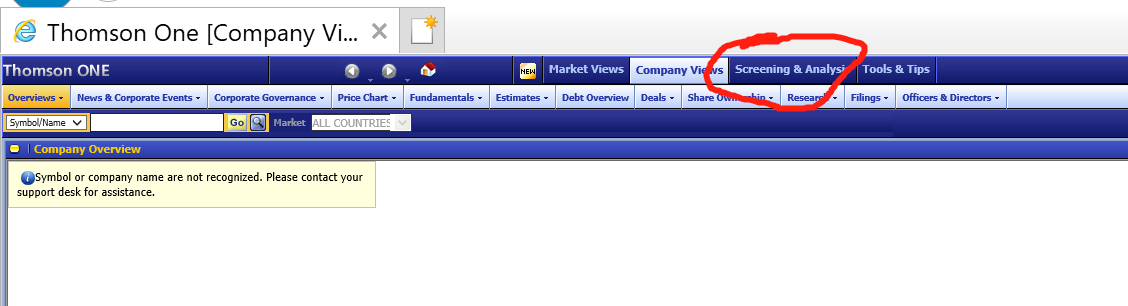
\includegraphics[width=.7\textwidth]{Figures/open_step1.png}
	\end{center}
	\end{figure}
	\begin{figure}[H]
	\begin{center}
	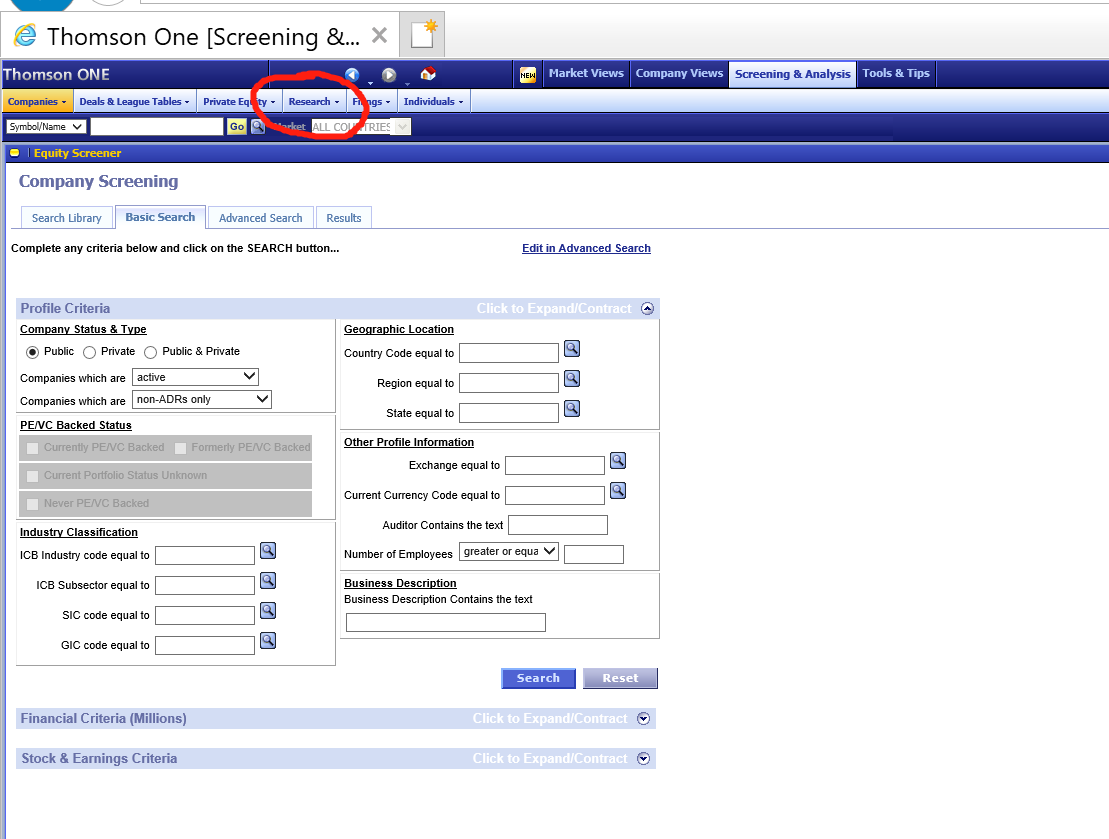
\includegraphics[width=.7\textwidth]{Figures/open_step2.png}
	\end{center}
	\end{figure}
	\item Put \textit{Streetevents} in the \textit{Contributor} field and choose \textit{Thomson Reuters Streetevents} in the drop-down list.
	\item Enter in \textit{Start Date} and \textit{End Date} to decide the scope of conference calls. Then press \textit{Enter}.
	\begin{figure}[H]
	\begin{center}
	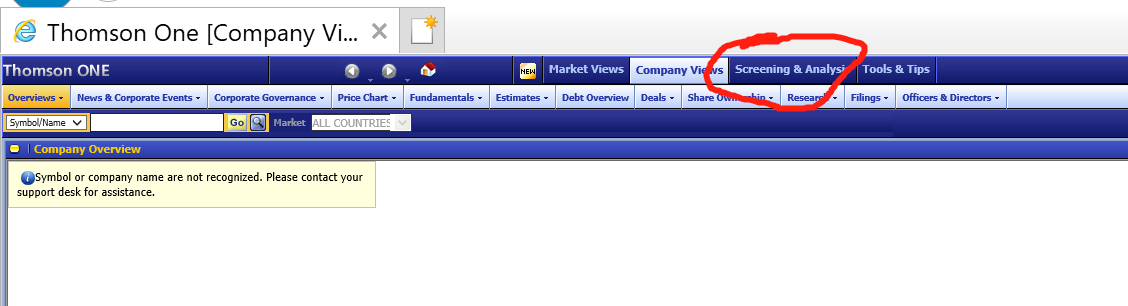
\includegraphics[width=.7\textwidth]{Figures/open_step1.png}
	\end{center}
	\end{figure}
	\begin{figure}[H]
	\begin{center}
	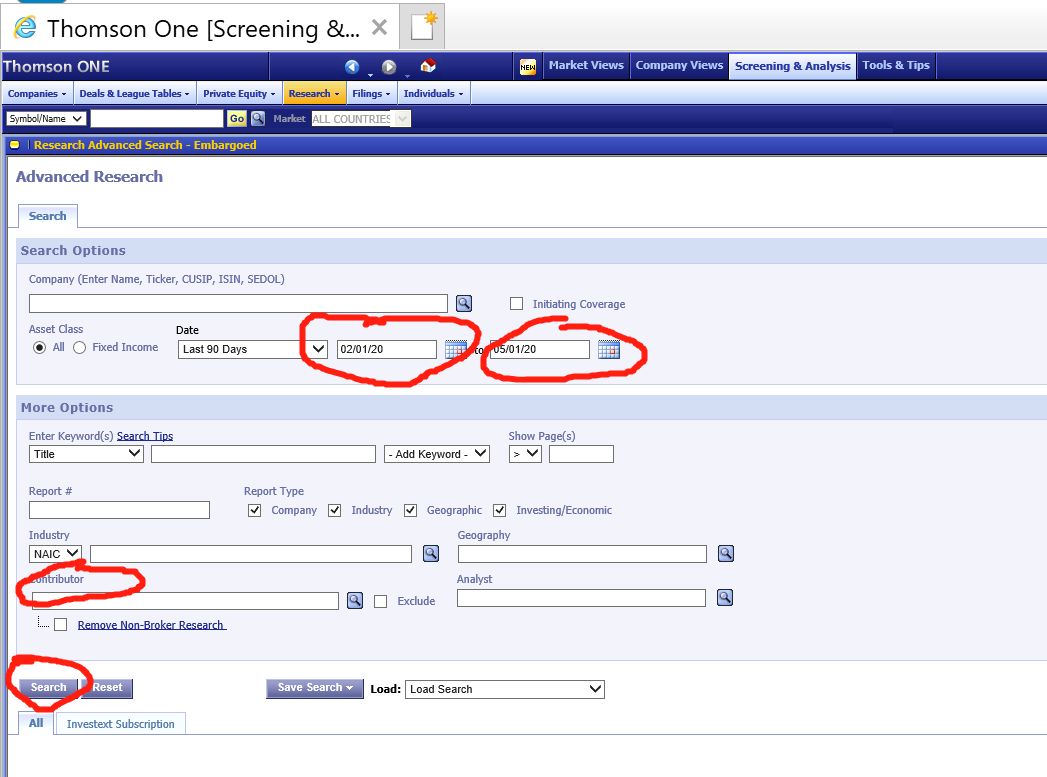
\includegraphics[width=.7\textwidth]{Figures/open_step3.png}
	\end{center}
	\end{figure}
\end{enumerate}
\par We use Python to download all the calls by using \textit{pynput} package to automatically control the mouse and keyboard. The main code is automatic\_download.py. mouse\_key\_recorder.py is a functional code that keeps record of the coordinates of positions that the mouse should click on. supplement\_download.py takes a predetermined list as the input, and the downloading process is the same as the main automatic code.
\par The automatic code follows the steps below:
\begin{enumerate}
	\item Enter start-time and end-time. We specify a four-day time period to ensure that each search gives no more than 2,000 calls. In round 2 and round 3 updates, since the number of conference calls is limited, we increase the time period. 
	\item Copy the number of calls given by the search, save the number into a separate data set, and calculate the pages.
	\item Select all calls in one page, download the pdf with all calls in that page, together with an excel which contains information of each call.\footnote{For each unit of observation in the excel, we have important variables including report number (unique identifier), report title (contains firm name) and date. This list is helpful in our parsing of the transformed pdf later on.} Also, to ensure that pdf and xls files are in pairs, we will check the existence of files in the folders. If there are some errors, the code will restart the process (by typing in the login websites, and automatically finishing the access steps. This is also the error handle step for any other errors).
	\item Uncheck all calls, click next page, repeat Step 2 and Step 3. If this is the last page of the date period, back to Step 1 with date moving backwards.\footnote{For all the mouse positions, we manually do one loop and use mouse\_key\_recorder.py to return a list of useful mouse positions.}
	\begin{figure}[H]
	\begin{center}
	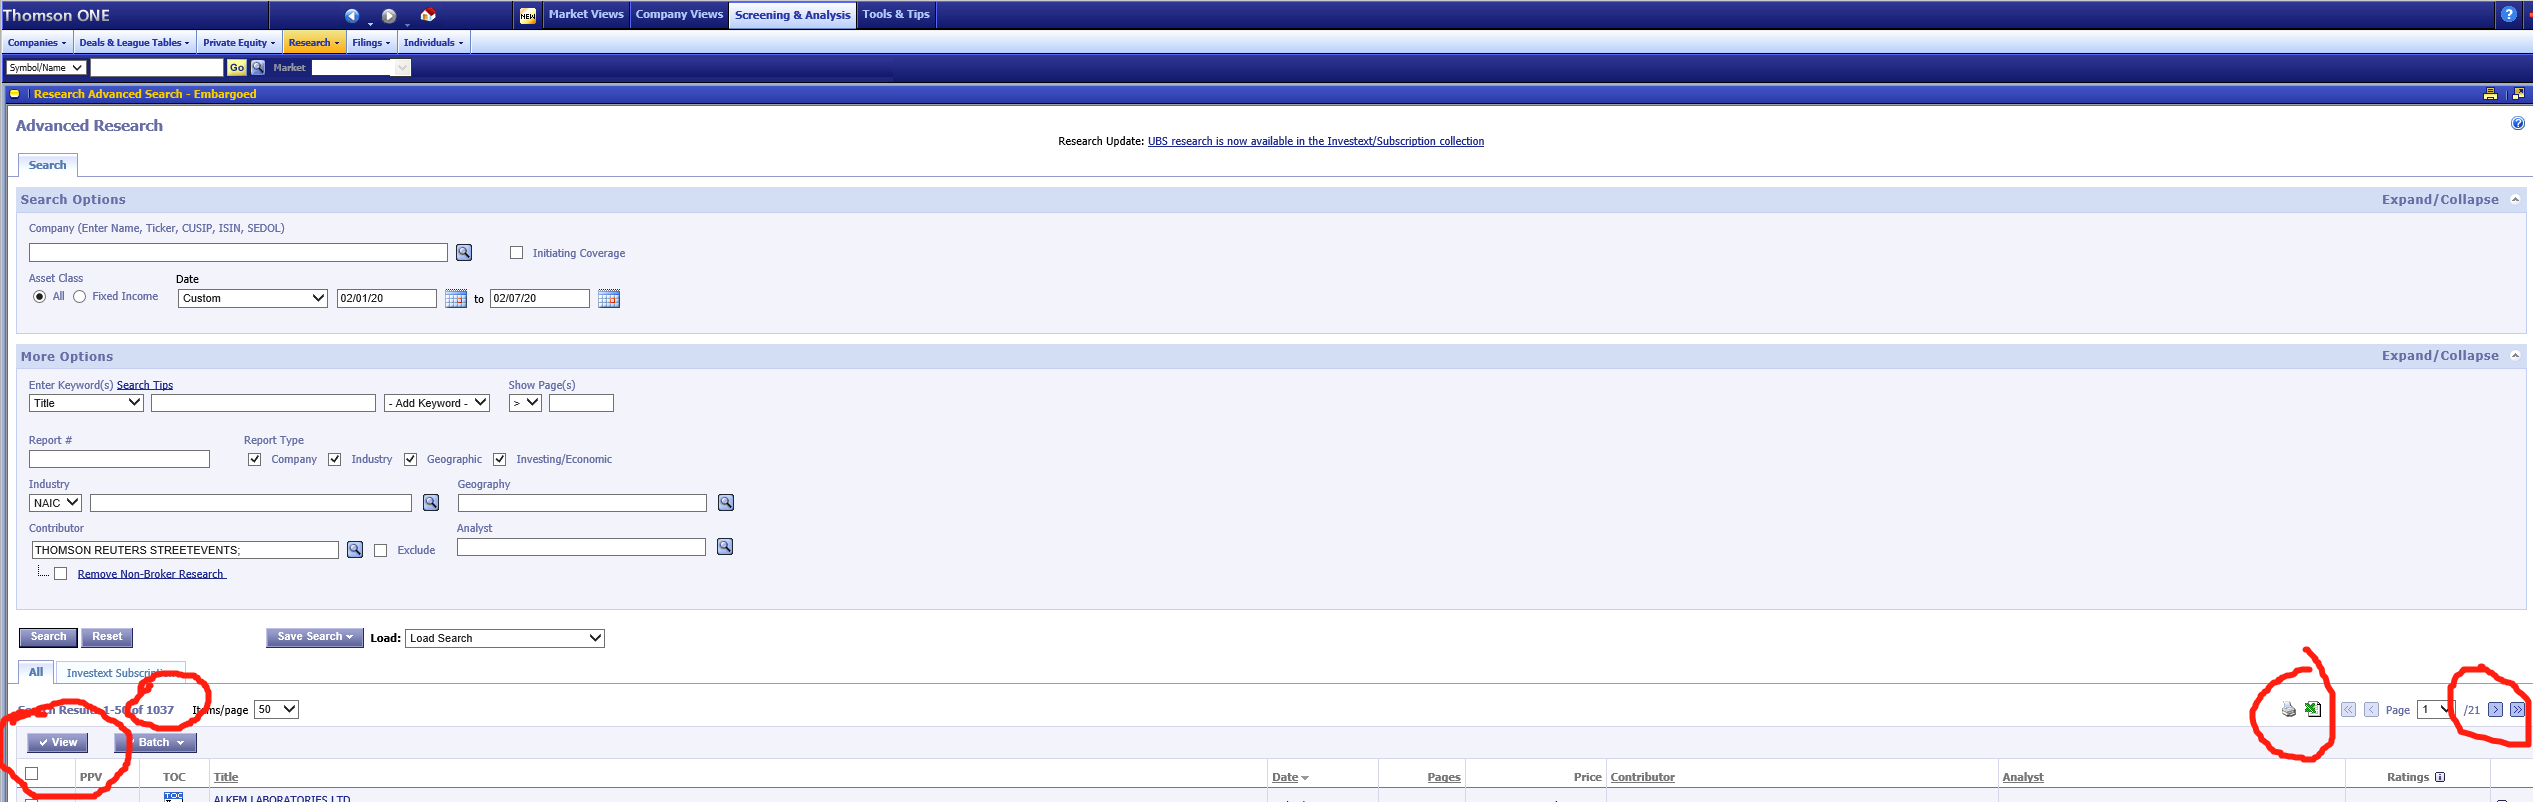
\includegraphics[width=.7\textwidth]{Figures/open_step4.png}
	\end{center}
	\end{figure}
\end{enumerate}
\par The automatic download is always affected by the network condition, and also Thomson One will automatically log off from time to time. So we need to handle the errors listed below:
\begin{enumerate}
	\item Automatically log off.
	\item Broken pdf pages and unsuccessful excel download.
	\item Sudden network error.
	\item Authentication error of the system (failure to log in).
	\item The change of file orders when we re-enter the system. (when the time-off is long, e.g., several hours)
\end{enumerate}
\par For most errors, the automatic code will try to re-enter the system by finishing all the access steps and retrieving the download from the previous break point. For error 4, please stop the code and wait for hours before we could access the system again. For error 5, we download the pdf first and then the excel because the pdf takes longer to download while the excel is quick to get. However, if the error occurs when the pdf is exported without the excel, we suggest to delete the pdf (when the error occurs, there will be one unpaired pdf) and re-download it to ensure the files are paired (which is important for the later processing).
\par If you run the code on a new laptop, please make sure to change the parameters below in the code:
\begin{itemize}
	\item Make sure your computer is zoomed 100\% in the settings.
	\item Use the mouse key recorder to capture the coordinates of every position and put it in the automatic code. This means that you should manually click on the positions to finish the step and the code will record the position. The coordinates will be accurate only if your computer is zoomed 100\%.
	\item Set up start date and end date, as well as the time window.
	\item Set up the folders for the pdf and xls separately.
\end{itemize}
\par The output of this step are pdf files in the RawScripts, and xls files in the List.

\section{Step 2: PDF Processing}
\par The next big step is to process all the pdfs into usable data files. Note that one pdf contains many firms' calls, so another challenge is how to split one file into different calls.  To achieve this, we use code ParseCCpdf\_v1.jl and take the following steps:
\begin{enumerate}
	\item Use the \textit{pdftotext} tool from Mercury server to transfer pdfs (.pdf) to texts (.txt) file.\footnote{\textit{pdftotext} is an OCR-reading tool. Information could be found at \url{https://poppler.freedesktop.org/}.} This tool would add page and paragraph delimiters while parsing the original file, which brings convenience for the split of firms. You could directly use pdftransfer.sh to submit jobs on the server. Please make sure you change the directory to the place where all raw pdfs are located.
	\item Use Julia to split the texts file and construct a primary database which contains report information (in the downloaded excel files) and raw call scripts. Specifically, start from the delimiters contained in the .txt file to identify pages, then use \textit{title} and \textit{pages} in the information file to locate the beginning and end of each conference call.\footnote{For some transcripts, the texts are laid out in two columns in the same page. And during this process there are always small problems to be dealt with.} Generate a new variable in the information file to store the raw call scripts. The primary database is a collection of .csv files with the following important variables:
	\begin{itemize}
		\item \textbf{Title} (firm name), \textbf{Subtitle} (firm name, date, and whether final/primary transcripts)
		\item \textbf{Date}, \textbf{Pages} (the number of pages of the call)
		\item \textbf{Analyst} (analysts who collect these transcripts, different analysts have slightly different forms of transcripts.)
		\item \textbf{Report} (Unique report number)
		\item \textbf{Call} (Raw call transcripts)
	\end{itemize}
\end{enumerate}
\par The output of this step are txt files in the RawScripts, and csv files in the CsvScripts.

\section{Step 3: Firm Matching}
\par Another important part is to match firms with Compustat to get: i. GVKEY (unique firm identifier); ii. country information. The task isn't trivial since the name of firms doesn't have strict spelling for various reasons.
\par WRDS gives full assess to \href{https://wrds-web.wharton.upenn.edu/wrds/query_forms/navigation.cfm?navId=60}{"Compustat - Capital IQ"} database, which contains various datasets. We can search for data by using the web interface page or through \href{https://wrds-www.wharton.upenn.edu/pages/data/sas-studio-wrds/}{SAS-Studio web application}. SAS-Studio allows to have access to all raw data tables, which we are using by the following steps:
\begin{enumerate}
\item Open the SAS-studio web application: \href{https://wrds-www.wharton.upenn.edu/pages/data/sas-studio-wrds/}{https://wrds-www.wharton.upenn.edu/pages/data/sas-studio-wrds/}
\item All files are located at "Server Files and Folder" (to the right hand).
\item Captiliq auxiliary files are located at \textit{wrds/capitaliq/sasdata/helper}.
\item Each table can be download by clicking the right mouse button. Although, it's not good practice, due to high size of tables.
\item The best way to download data is to create Query (right mouse button on a table $\Rightarrow$ new $\Rightarrow$ Query). 
\item Downloading Query's result is a little bit tricky, since you can only print the result. The result is located in user's temporary folder. To find the name of the temporary folder: 1) open any table 2)push "display the code .." button 3) run the code 4) Result window $\rightarrow$ Engine/Host Dependent Information $\rightarrow$ filename shows your temporary folder. 
\end{enumerate}
\par We used the following tables with specific columns from Compustat:
\begin{enumerate}
	\item \textbf{CIQCOMPANY}: companyid, companyname, tickersymbol, countryid and other columns. Total: 24,511,757 obs. Public Companies: 66,256. Private Companies: 16,544,322. Public Investment Firms: 1,987 and Private Investment Firms: 203,407
	\item \textbf{WRDS\_GVKEY}: companyid, gvkey (115,357 observations).
	\item \textbf{CIQCOUNTRY}: countryid, countryname: countryid, countryname (221 countries).
\end{enumerate}
\par In addition, we have Hassan's Firm-Level Political Risk Dataset,\footnote{\href{https://www.firmlevelrisk.com/download}{Firm-Level Risk website.}}  which also provides us with GVKEY and firm names. We think that this data set contains almost all the company's names that we have, since we use the same data source.\footnote{In addition, in contrast to the Compustat dataset, Hassan's dataset has English spelling for all company's names, which helps us, since Conference Calls also has English spelling names. }  
\par We merged all tables into \textit{compustat\_company.csv}. This file contains \textit{company name, compnany id, gvkey, tickersymbol, countryid and countryname.} The data from Hassan are named as FirmSVkey.csv. These files are in AuxData inside firmMatchingCode. To match firms' names with Compustat, we now have three sources: Hassan's dataset, Compustat dataset, and unique Tickers. If several firms has the same ticker, we don't use the ticker on the "perfect matched" step. We use program code linkCCtoGvkey.jl and follow the steps described below:
\begin{enumerate}  
	\item Process firms' names: 1) lower alphabets. 2) delete all special symbols. 3) delete all common words.\footnote{We deleted the words: group, plc, ltd, limited, ag, corp, corporation, Incorporation, laboratories, labs, the, holdings, oyj, inc, conference call, conference, co, company, trust, investment, investments, sln, sa, event transcript of, event brief of., and others.}
	\item Match firms by three sources\footnote{The result table has three additional columns: \textit{gvkey\_t, gvkey\_h, gvkey\_c} which are for Ticker, Hassan and Compustat datasets matching.} and combine all results. This is "Perfect Match" step, since we haven't used any guess method yet.
	\item For the remaining unmatched firms, we use compare-function, which is based on Jaro string distance and return the probability that the two string are equal. First, we match firms with the same ticker (38\% of a subset) and keep the best guess of a name if the probability is higher than 80\%.\footnote{We have checked that 80\% is enough for matching names with the same ticker.} After that, the firm is matched with all possible names from Compustat and Hassan's dataset.\footnote{Matched name and probability is saved into columns \textit{gues\_name and prob}.} We can sure about matched name with probability above 90\%.
\end{enumerate}
\par The output of this step are the firm matching csvs in FirmNameMatching.


\section{Summary of Textual Analysis Practices}
\par After we obtain the cleaning conference call scripts, we implement a series of textual analysis practices. We give a brief summary of the practices, with some tips on processing the large scale text data.
\par We replicated the main analysis in \href{https://drive.google.com/file/d/1D7wNA31oltU4yndcLWw3Eo3LPJltEXg_/view?usp=sharing}{Hassan et al. (2019)} and calculated the political risk index for each company at the quarter level. We'll not talk about the details, but more about the general tips in speeding up the practice. This includes:
\begin{enumerate}
	\item We use multi-process and multi-core to improve speed both in Python and Julia. However, this is not the main solution since Booth server has very limited source for high-memory nodes. Additionally, you may have to wait in queue on the server, which makes multi-process and multi-core slower than you may expect.
	\item An account could submit up to 150 batch jobs on the server. And if the job is in parallel, i.e., you do not need to feed the whole data set to one code, it is always the best way to separate the data sets into smaller ones, and create various batch files taking numeric inputs. For example, in our political risk index replication, the main task is to use dictionary-based metrics to model the risk. Every conference call is relatively independent. For term frequency, we could also sum up the statistics for smaller data sets. As a result, we first automatically separate the csv files into 50 different folders (you may use more or fewer folders, 50 is good for us in this set of practice), and then separately calculate the index for each folder. The submit batch file will take the order 1-50 as the input for Python codes. This helps a lot in speeding things up. (Also, for these batch files, since they varies only in directory and numeric order, we use Python codes to generate them in bulk)
	\item We use widely-used packages including nltk, SpaCy, sklearn, gensim for Python. For LDA practice, we use a simple package topic-modelling-tools for Collapsed Gibbs Sampling estimation, and use a faster version of online Variational Bayesian algorithm from \href{https://github.com/blei-lab/onlineldavb}{Blei}. For the latter package, we make adjustments on the source code to generate ideal outcomes and diagnostics.
\end{enumerate}
\par Now you could probably imagine the output of any textual analysis practices. The final data set will be at the conference call level, with the firm name from firm matching results (and gvkey to link to other firm data sets), and the main textual analysis index. For topic modelling, the outcome will be a vector of topic distribution for every conference call. In addition to the aforementioned political risk index, we also try several keyword-based methods, and sentiment analysis on conference call scripts.

\end{document}
